%%%%%%%%%%%%%%%%%%%%%%%%%%%%%%%%%%%%%%%%%%%%%%%%%%%%%%%%%%%%%%%%%%%%%%%%%%%%%%%%
%2345678901234567890123456789012345678901234567890123456789012345678901234567890
%        1         2         3         4         5         6         7         8
\documentclass[letterpaper, 10 pt, conference]{ieeeconf}  % Comment this line out
                                                          % if you need a4paper
%\documentclass[a4paper, 10pt, conference]{ieeeconf}      % Use this line for a4

\usepackage{float}
                                                          % paper
% uso paquete bookmark para tener bien los outlines.
\usepackage{bookmark}

% Configuro el idioma.
\usepackage[utf8]{inputenc} % Importante para mantener acentos.
\usepackage[spanish, activeacute]{babel} % Requiere: texlive-lang-spanish. Por primera vez hay que ejecutar: texconfig init> log

% Paquete para poder usar acentos en $$.
\usepackage{mathtools}
%\setmathfont{XITS math}

% Para los diagramas de flujo
\usepackage{tikz}
\usetikzlibrary{shapes.geometric, arrows}

% Elementos del diagrama
\tikzstyle{startstop} = [rectangle, rounded corners, 
minimum width=6em, 
minimum height=2em,
text centered, 
draw=black, 
fill=red!30]

\tikzstyle{io} = [trapezium, 
trapezium stretches=true, % A later addition
trapezium left angle=70, 
trapezium right angle=110, 
minimum width=6em, 
minimum height=2em, text centered, 
draw=black, fill=blue!30]

\tikzstyle{block} = [rectangle, 
minimum width=8em, 
minimum height=3em, 
text centered, 
text width=7.5em, 
draw=black, 
fill=white!30]

\tikzstyle{def} = [rectangle, 
minimum width=14em, 
minimum height=3em, 
text centered, 
text width=12em, 
draw=black, 
fill=purple!30]

\tikzstyle{swap_proccess} = [rectangle, 
minimum width=8em, 
minimum height=2em, 
text centered, 
text width=8em, 
draw=black, 
fill=orange!30]

\tikzstyle{process} = [rectangle, 
minimum width=6em, 
minimum height=2em, 
text centered, 
text width=6em, 
draw=black, 
fill=orange!30]

\tikzstyle{decision} = [diamond, 
minimum width=6em, 
minimum height=6em, 
text centered, 
draw=black, 
fill=green!30]
\tikzstyle{arrow} = [thick,->,>=stealth]

\usepackage{siunitx}

% package to get \url
\usepackage{hyperref}
\hypersetup{
  colorlinks=true,
  linkcolor=magenta,
  filecolor=magenta,
  citecolor=magenta,      
  urlcolor=magenta,
}

% Graficos electrónicos
\usepackage[RPvoltages]{circuitikz}

\IEEEoverridecommandlockouts                              % This command is only
                                                          % needed if you want to
                                                          % use the \thanks command
\overrideIEEEmargins
% See the \addtolength command later in the file to balance the column lengths
% on the last page of the document

\usepackage{graphicx}
\usepackage{graphics}

% styling for matlab/octave code.
\usepackage{matlab-prettifier}
% Configuracion, con esto puede agregar ñ.
\lstset{
  literate={ñ}{{\~n}}1
}

\usepackage{listings}

% The following packages can be found on http:\\www.ctan.org
%\usepackage{graphics} % for pdf, bitmapped graphics files
%\usepackage{epsfig} % for postscript graphics files
%\usepackage{mathptmx} % assumes new font selection scheme installed
%\usepackage{times} % assumes new font selection scheme installed
\usepackage{amsmath} % assumes amsmath package installed
%\usepackage{amssymb}  % assumes amsmath package installed

\title{\LARGE \bf Trabajo Práctico N° 1 Ejercicio 3}

\author{
  Tom\'as Vidal\\
  {\it Control de sistemas biológicos}\\
  {\it Facultad de Ingenier\'ia, UNLP, La Plata, Argentina.}\\
  {\it 18 de Septiembre, 2024.}
}                                            % <-this % stops a space
% comienzo
% INTRO

% Figura
\newcommand{\image}[2] {
  \begin{figure}[H]
    \centering
    \includegraphics[width=0.43\textwidth]{./#1.png}
    \caption{#2}
    \label{fig:#1}
  \end{figure}
}

% Codigo
% \begin{lstlisting}[style=Matlab-editor]
% % el código va aca
% dispc("HELLO WORLD");
% \end{lstlisting}

\begin{document}
% - - - - - - - - - - - - - - - - - - - - - - - - - - - - - -  TITLE
\begin{titlepage}
	\centering
	\null\vspace{4cm} % Adjust this value to push everything down
	{\LARGE \textbf{Trabajo Práctico N° 2} \par}
	\vspace{2cm}
	{\large Tomás Vidal \par}
	{\itshape Control de sistemas biológicos \par}
	{\itshape Facultad de Ingeniería, UNLP, La Plata, Argentina. \par}
	{\itshape 18 de Mayo, 2025. \par}
	\vspace{2cm}
	
\includegraphics[width=0.55\textwidth]{unlp_logo.png}
	\vfill % Pushes the content to properly center vertically
\end{titlepage}
% - - - - - - - - - - - - - - - - - - - - - - - - - - - - - -

\section{Introducción}

En el control de sistemas biológicos, la estimación precisa de variables no medibles (\textit{como la concentración de sustrato}) es esencial para optimizar procesos como la producción de plásticos. Este informe evalúa tres estrategias de observación:

\begin{itemize}
  \item{Observador exponencial: Basado en ajuste de polos, sensible a variaciones paramétricas pero de fácil implementación.}
  \item{Observador de Kalman Extendido (EKF): Óptimo bajo incertidumbre, minimiza error cuadrático mediante la ecuación de Riccati.}
  \item{Observador asintótico: Independiente del modelo (excepto $K_{s2}$), robusto y de convergencia exacta.}
\end{itemize}

Cada método fue validado bajo perturbaciones paramétricas (40\%) y de dilución, analizando su error transitorio, convergencia y robustez. Los resultados permitirán seleccionar la técnica más adecuada para aplicaciones reales.

\section{Observador exponencial}

En el marco del sistema biológico analizado en el Trabajo N°1 (PHB), en la etapa de producción de plástico, se implementó un observador exponencial para estimar la concentración de sustrato a partir de mediciones de la concentración de plástico producido. \\
La sintonización de los polos del observador se realizó mediante un proceso iterativo, evaluando diferentes configuraciones hasta alcanzar un equilibrio entre velocidad de convergencia y robustez. Si bien este método no es óptimo desde un punto de vista analítico, permitió identificar una configuración adecuada para minimizar el error de estimación.

\begin{figure}[H]
  \centering
  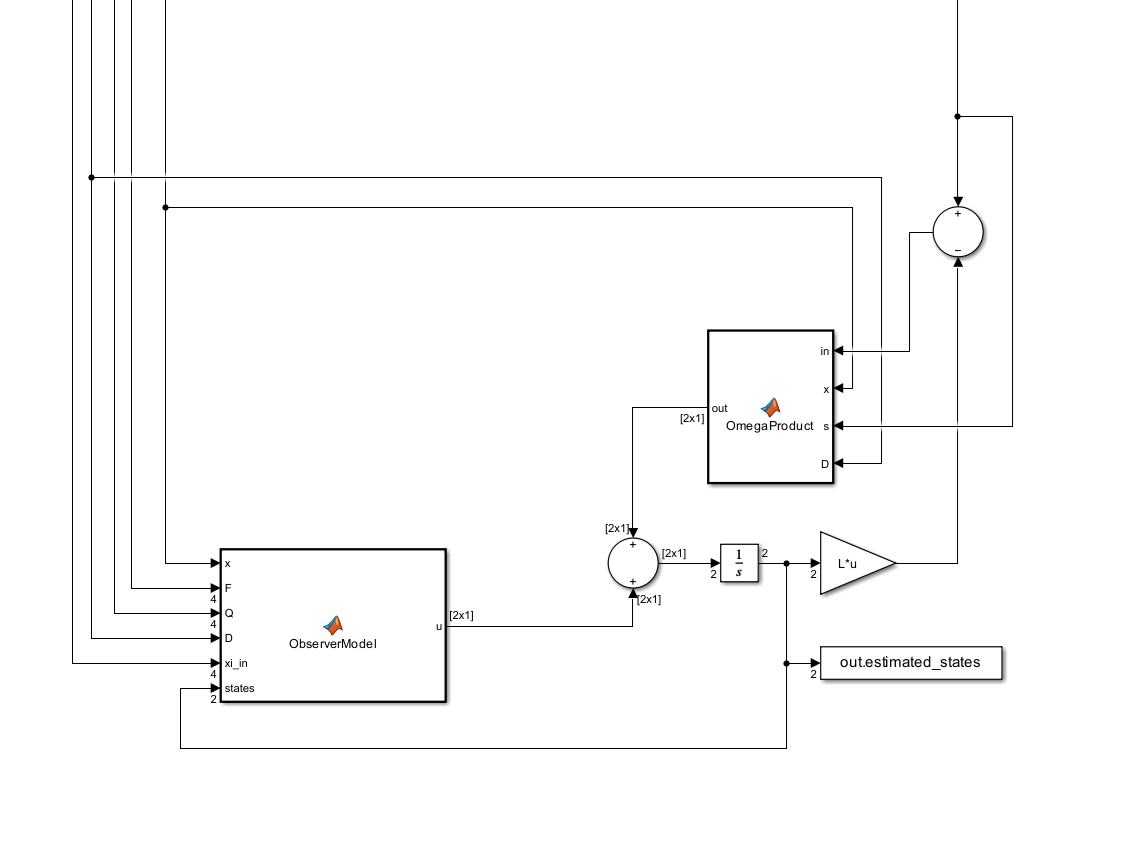
\includegraphics[width=0.43\textwidth]{./Images_tp2/estimadorExponencial.png}
  \caption{Simulink del estimador exponencial}
\end{figure}

\subsection{Validación y Análisis de Robustez}

Para validar el desempeño del observador, se comparó la estimación del sustrato con los valores ``reales'' generados por el modelo de referencia. El error relativo demostró una convergencia aceptable en régimen permanente, aunque se observaron desviaciones durante la fase transitoria.

Adicionalmente, se evaluó la robustez del observador ante variaciones paramétricas en su modelo interno, al igual que el rechazo a perturbaciones haciendo una variación de la dilución (D). Las gráficas de estimación bajo perturbaciones revelaron que:

\begin{itemize}
    \item{La dinámica transitoria del sustrato estimado es altamente sensible a cambios en los parámetros del observador.}
    \item{A pesar de estas variaciones, el observador mantiene su capacidad de converger al valor real en estado estacionario, lo que sugiere que el diseño es consistente en régimen permanente pero requiere ajustes finos para mejorar la respuesta transitoria.}
\end{itemize}

\begin{figure}[H]
  \centering
  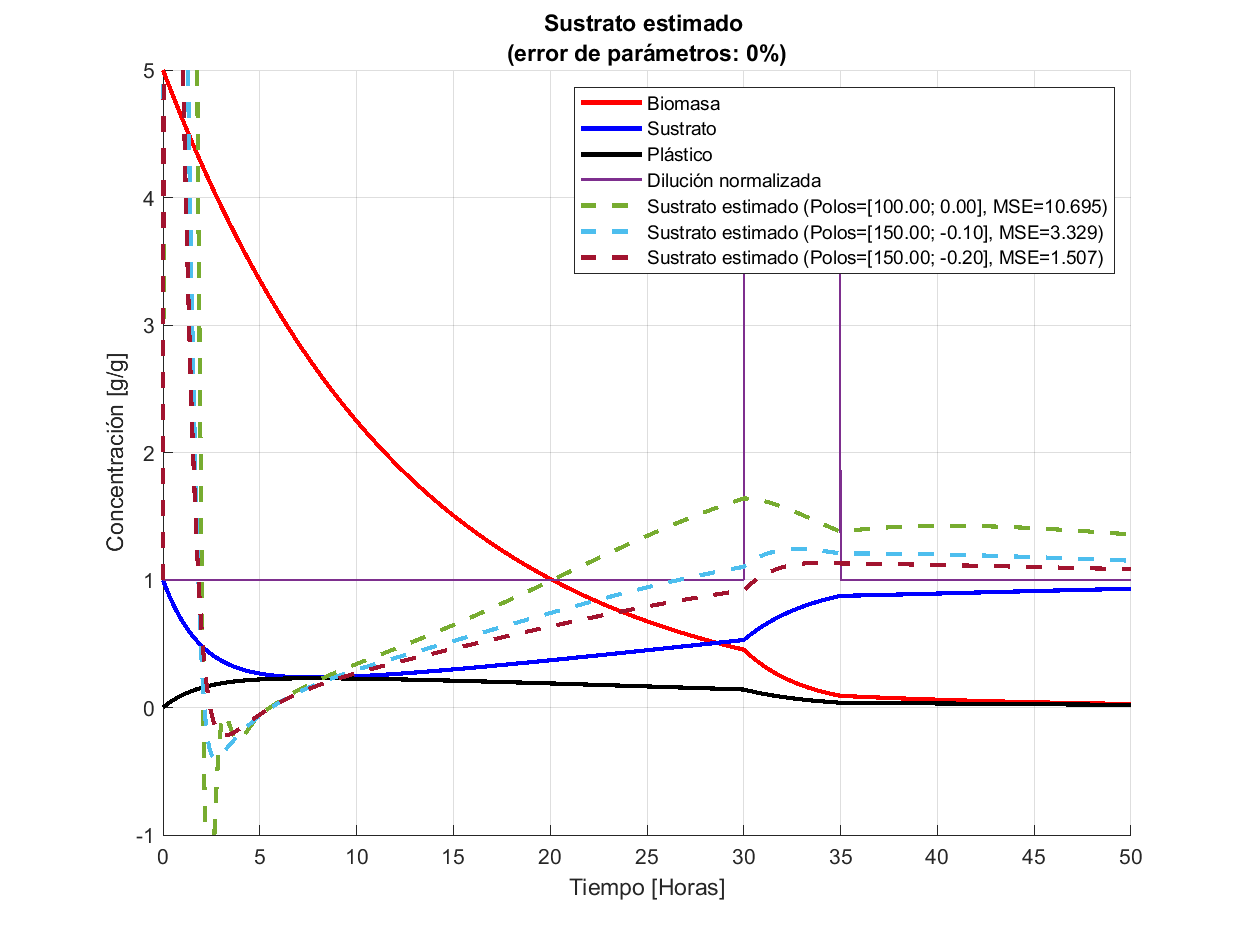
\includegraphics[width=0.43\textwidth]{./Images_tp2/exponencial_1.png}
  \caption{Observador exponencial sin errores de parámetros}
\end{figure}

\begin{figure}[H]
  \centering
  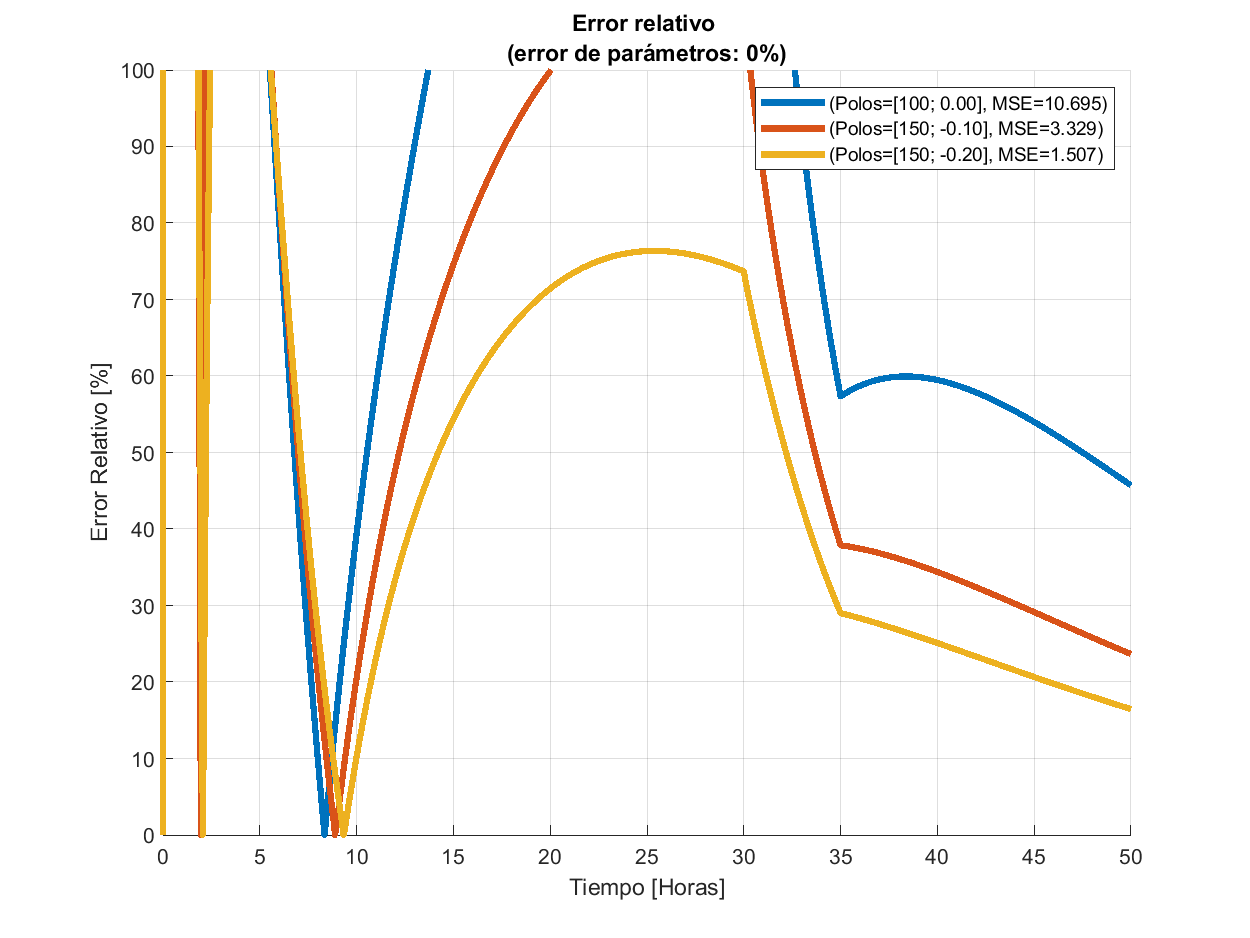
\includegraphics[width=0.43\textwidth]{./Images_tp2/exponencial_1_error.png}
  \caption{Error relativo del observador exponencial sin errores de parámetros}
\end{figure}

\begin{figure}[H]
  \centering
  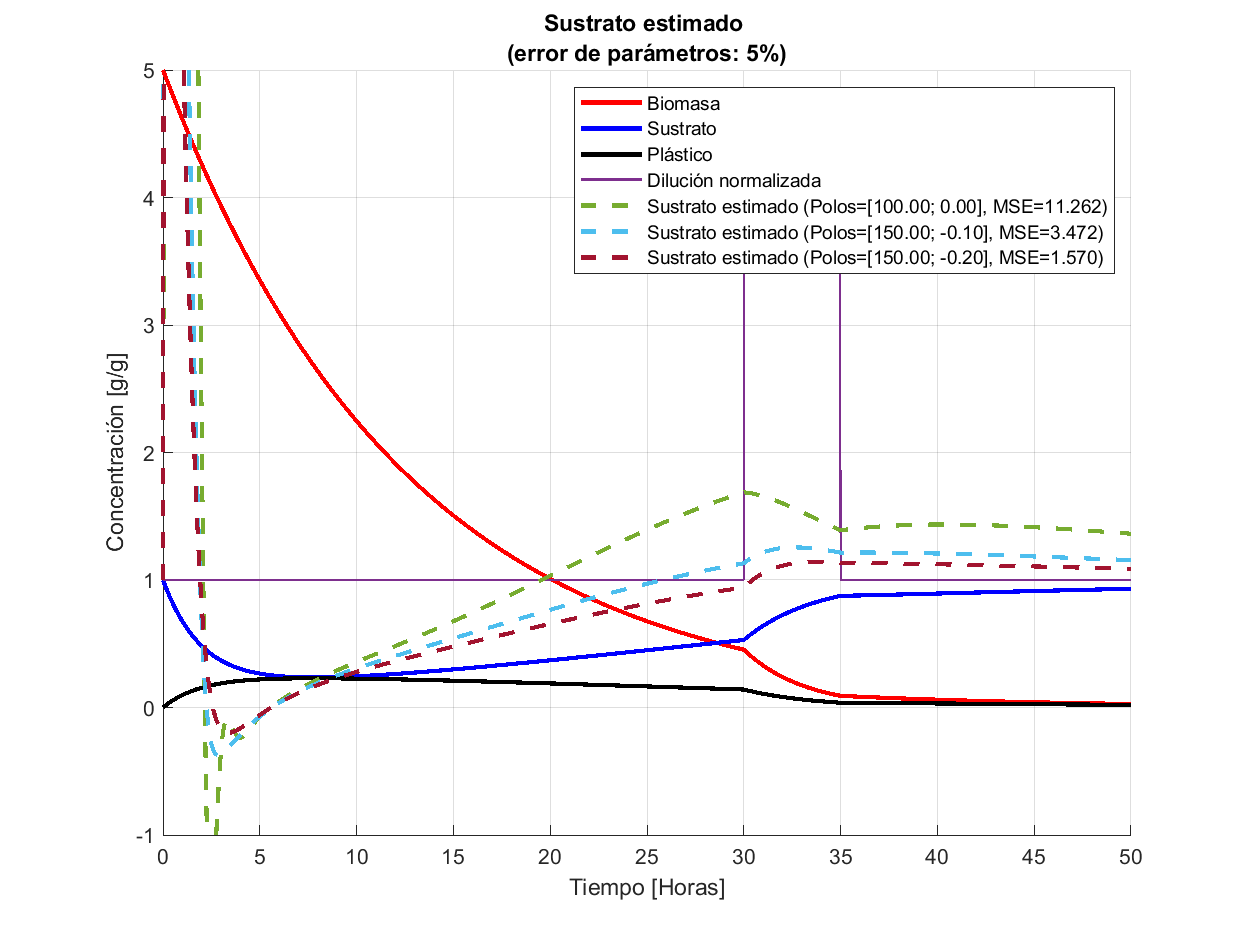
\includegraphics[width=0.43\textwidth]{./Images_tp2/exponencial_2.png}
  \caption{Observador exponencial con error de parámetros al 5\%}
\end{figure}

\begin{figure}[H]
  \centering
  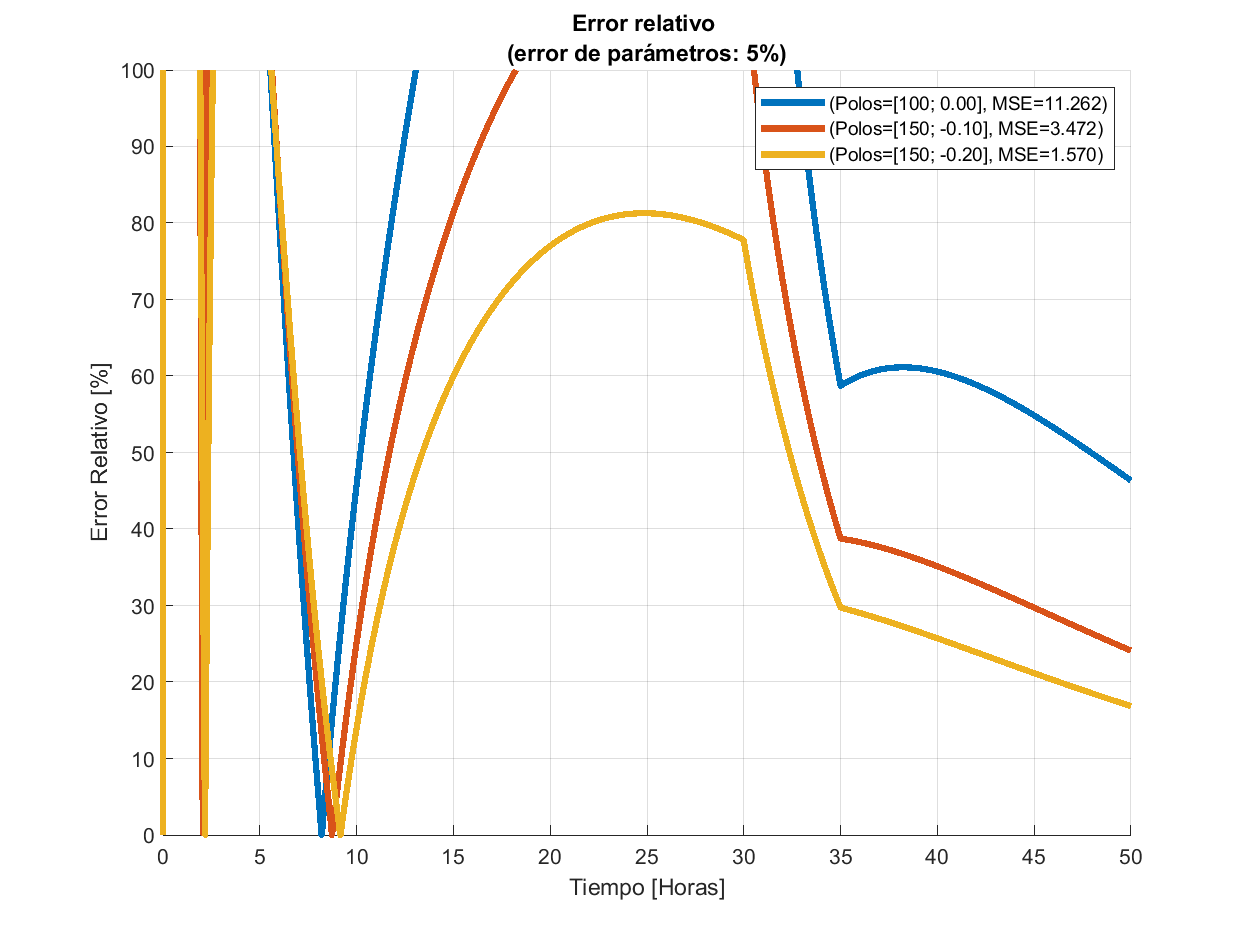
\includegraphics[width=0.43\textwidth]{./Images_tp2/exponencial_2_error.png}
  \caption{Error relativo del observador exponencial con error de parámetros al 5\%}
\end{figure}

\begin{figure}[H]
  \centering
  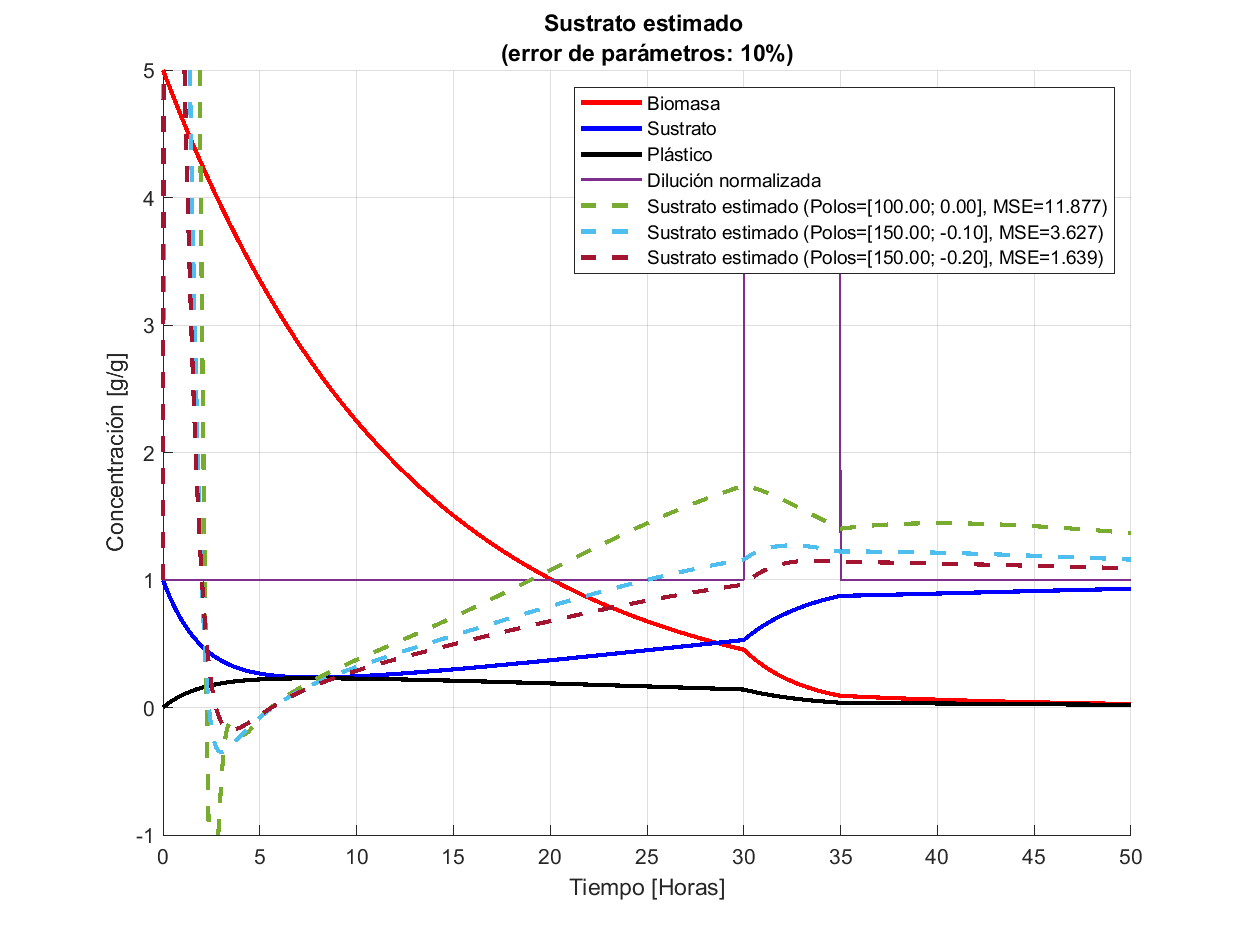
\includegraphics[width=0.43\textwidth]{./Images_tp2/exponencial_3.png}
  \caption{Observador exponencial con error de parámetros al 10\%}
\end{figure}

\begin{figure}[H]
  \centering
  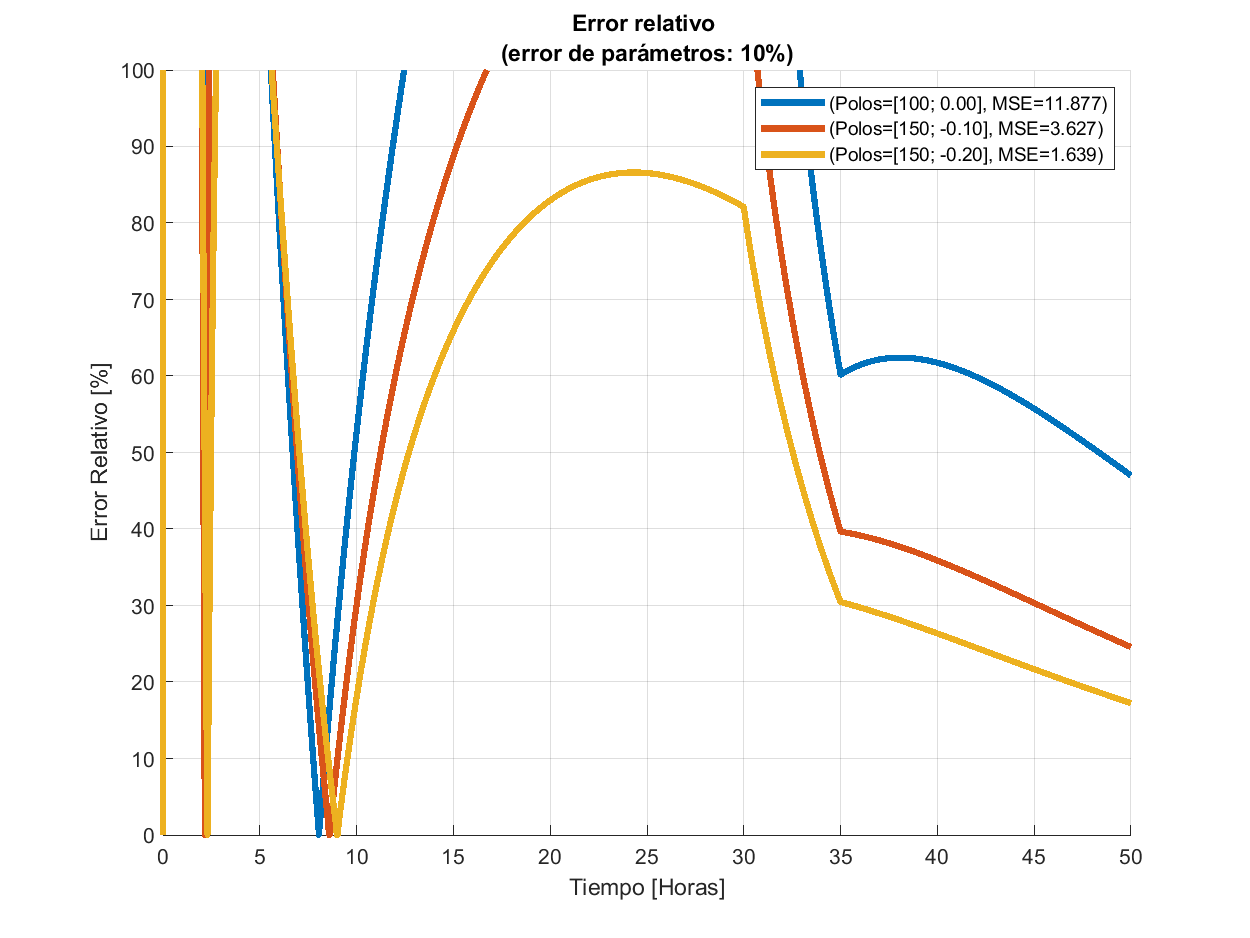
\includegraphics[width=0.43\textwidth]{./Images_tp2/exponencial_3_error.png}
  \caption{Error relativo del observador exponencial con error de parámetros al 10\%}
\end{figure}

\begin{figure}[H]
  \centering
  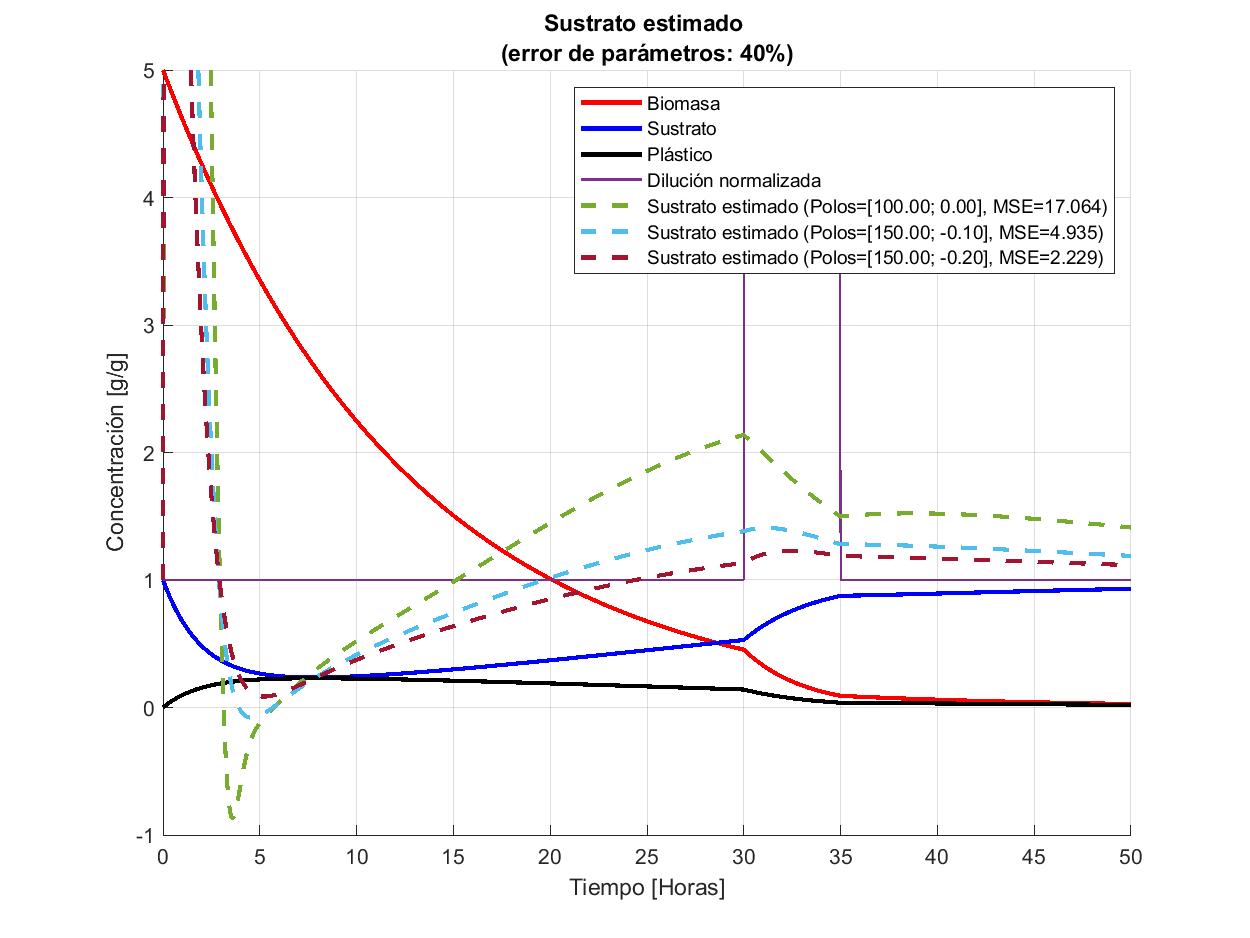
\includegraphics[width=0.43\textwidth]{./Images_tp2/exponencial_4.png}
  \caption{Observador exponencial con error de parámetros al 40\%}
\end{figure}

\begin{figure}[H]
  \centering
  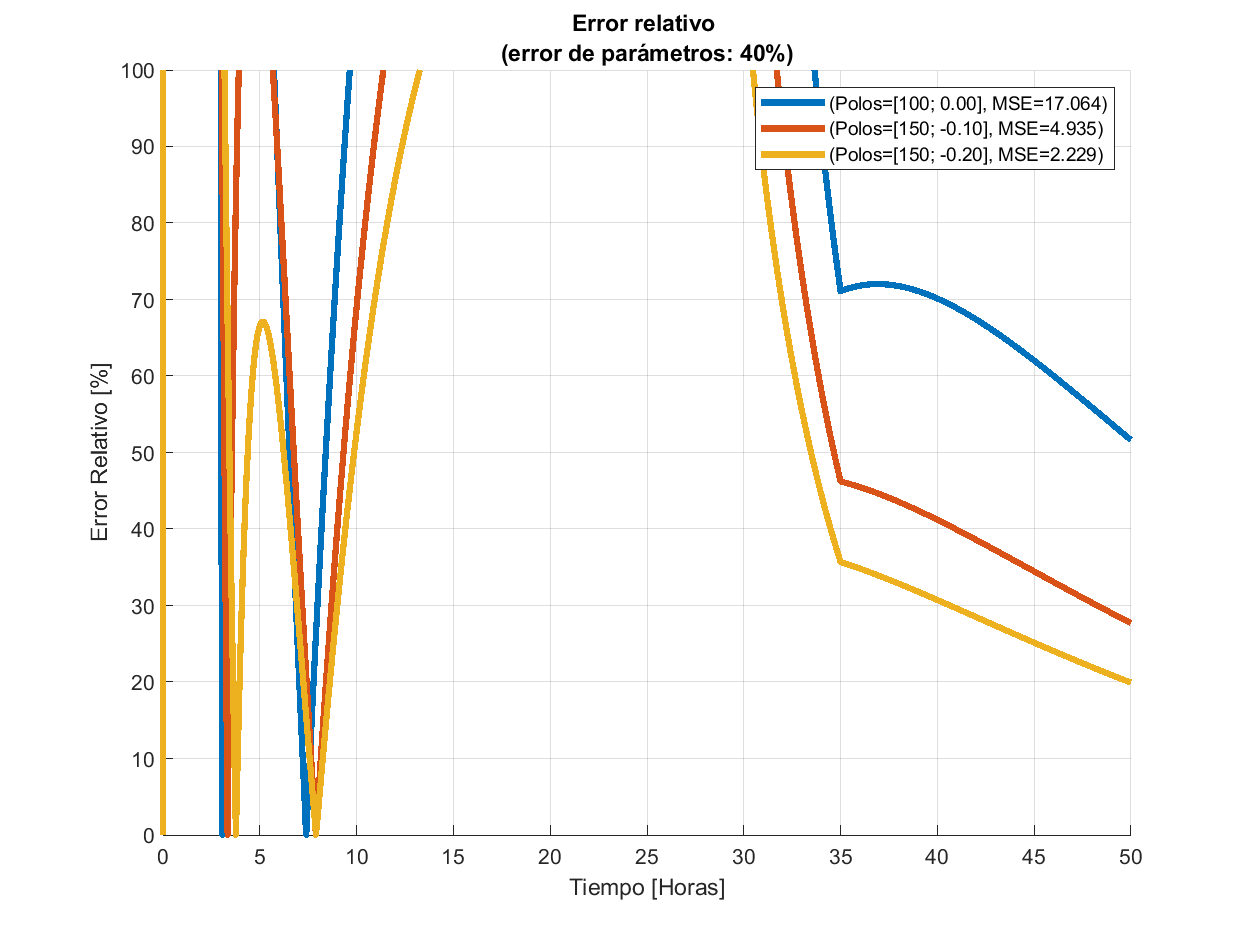
\includegraphics[width=0.43\textwidth]{./Images_tp2/exponencial_4_error.png}
  \caption{Error relativo del observador exponencial con error de parámetros al 30\%}
\end{figure}

\section{Observador de Kalman}

Se implementó un Observador de Kalman Extendido (EKF), el cual utiliza un enfoque estocástico para optimizar la ganancia del observador mediante la solución de la ecuación de Riccati. A diferencia del observador exponencial (que ajusta polos de forma heurística), el EKF minimiza una función de error cuadrático, proporcionando estimaciones óptimas en el sentido de mínima varianza.

Los resultados muestran que el EKF reconstruye con precisión la concentración de sustrato, incluso superando al observador exponencial en velocidad de convergencia y suavidad de la estimación.

Para evaluar robustez, al igual que antes, se introdujeron variaciones paramétricas de hasta 40\% en los parámetros del modelo interno del observador, al igual que una perturbación en la dilución (D) para evaluar el rechazo a perturbaciones. Se observó que:

\begin{figure}[H]
  \centering
  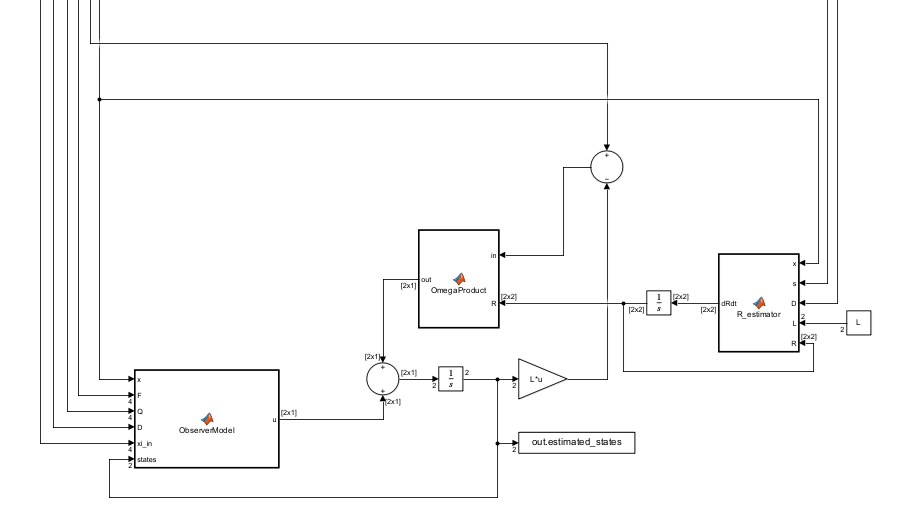
\includegraphics[width=0.43\textwidth]{./Images_tp2/simulink_kalman.png}
  \caption{Simulink observador de Kalman}
\end{figure}

\begin{itemize}
  \item{Efecto en el transitorio: Las desviaciones paramétricas afectan la dinámica inicial, generando sobre/subestimaciones durante la fase transitoria.}
  \item{Convergencia en régimen permanente: A pesar de las perturbaciones, el EKF mantiene su capacidad de converger al valor real, gracias a la corrección recursiva basada en las mediciones.}
\end{itemize}

\begin{figure}[H]
  \centering
  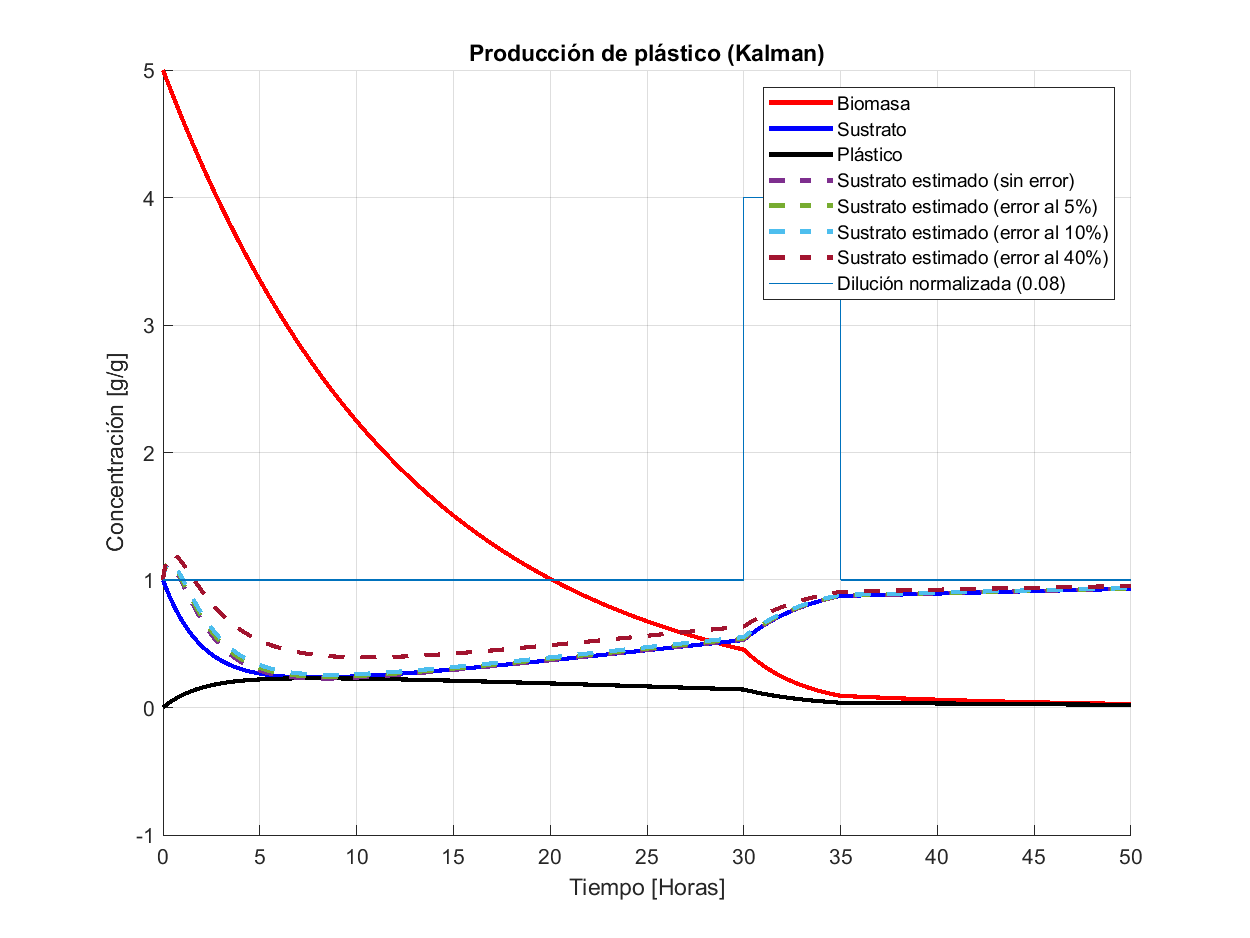
\includegraphics[width=0.43\textwidth]{./Images_tp2/kalman.png}
  \caption{Observador de Kalman para diferentes variaciones de parámetros}
\end{figure}

\begin{figure}[H]
  \centering
  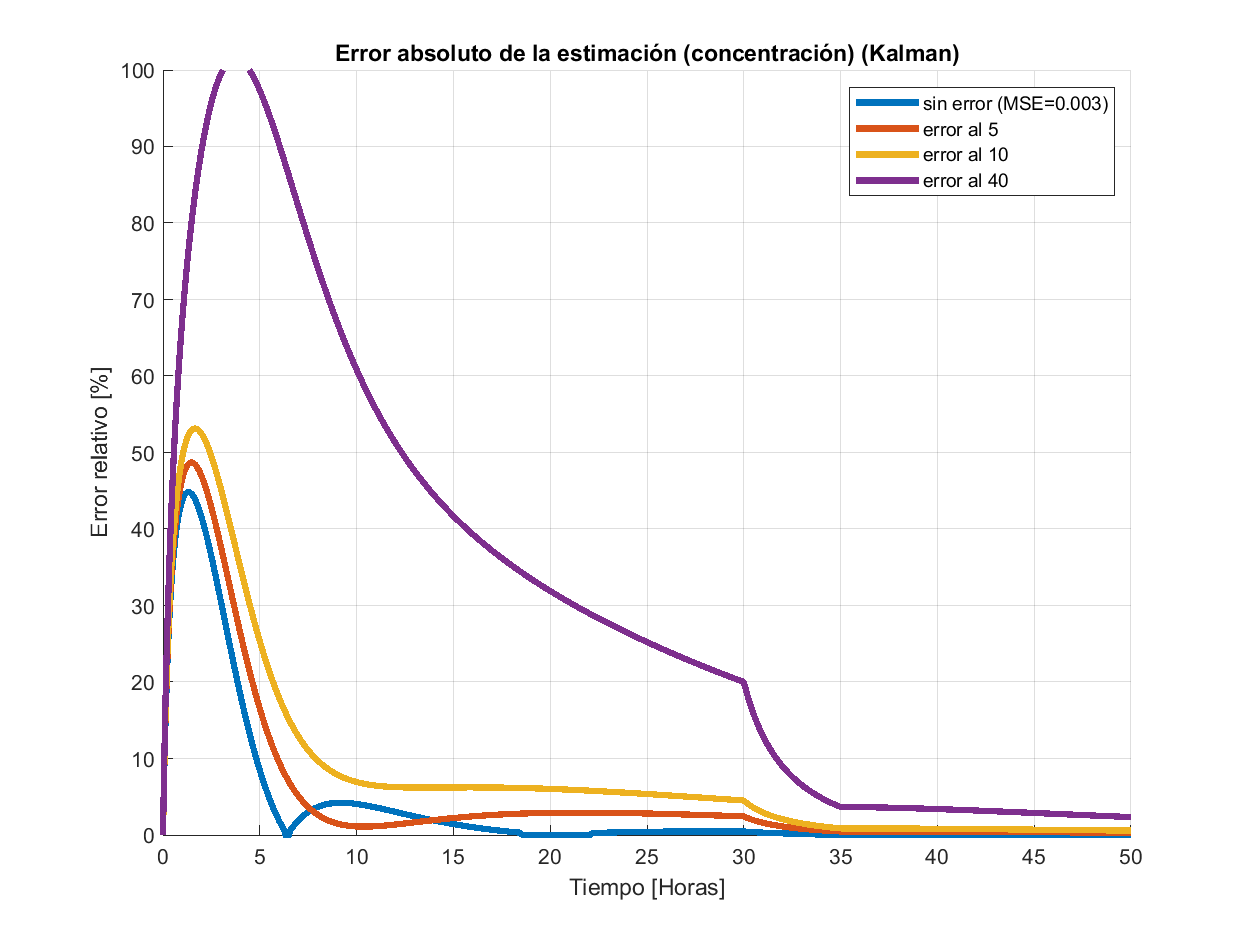
\includegraphics[width=0.43\textwidth]{./Images_tp2/kalman_error.png}
  \caption{Errores relativos del observador de Kalman}
\end{figure}


\section{Observador asintótico}

A diferencia de los observadores basados en modelos (exponencial y Kalman extendido), el observador asintótico emplea un cambio de variable matemático para reconstruir la concentración de sustrato sin depender explícitamente de la dinámica del sistema, excepto por el parámetro Ks2Ks2​ (asociado a la cinética del proceso). Este enfoque lo hace particularmente robusto frente a incertidumbres en los demás parámetros del modelo.

\begin{equation*}
  \dot{s} = -K_{s2} * r_{p} + D(S_{in} - s) \\
\end{equation*}

\begin{equation*}
  \dot{p} = 1 * r_{p} + D(-s)
\end{equation*}

Con la transformación:

\begin{equation*}
  z = A_{0} * p + s
\end{equation*}

\begin{equation*}
  A_{0} = K_{s2}
\end{equation*}

Por lo que el estimador resulta:

\begin{equation*}
  \hat{s} = \hat{z} - K_{s2} * p
\end{equation*}

\begin{figure}[H]
  \centering
  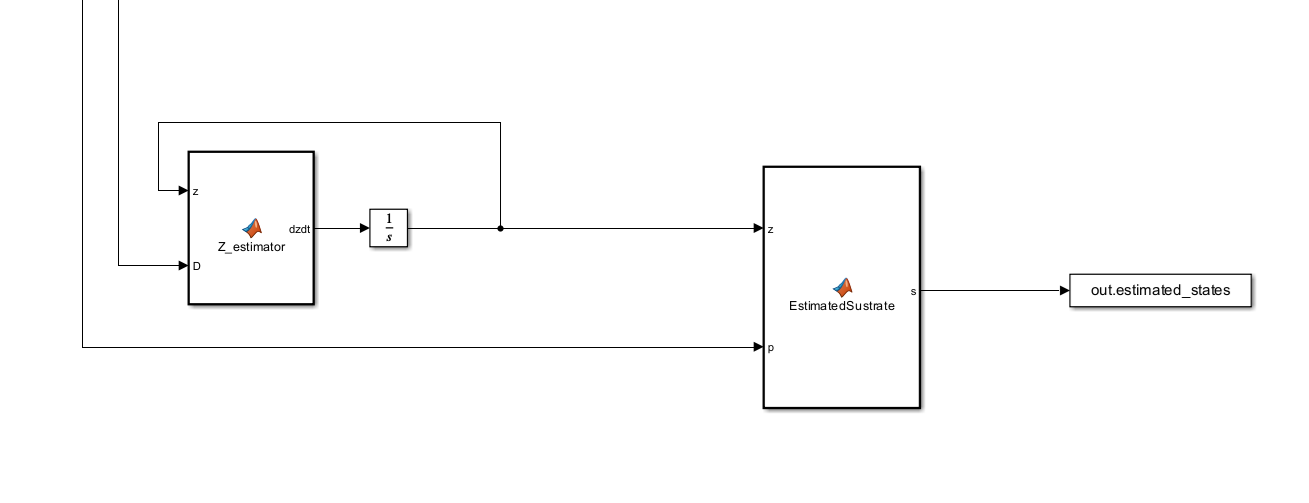
\includegraphics[width=0.43\textwidth]{./Images_tp2/simulink_asintotico.png}
  \caption{Simulink del observador asintotico}
\end{figure}

Para evaluar el desempeño del observador asintótico, se realizaron pruebas bajo dos escenarios, al igual que antes:

\begin{itemize}
  \item{Variación paramétrica de $K_{s2}$ (hasta 40\%)}
  \item{Perturbaciones en la tasa de dilución (cambios abruptos en el flujo de entrada/salida).}
\end{itemize}

\subsection{Resultados clave}

\begin{itemize}
  \item{Convergencia exacta en estado estacionario: El error de estimación tiende a cero, al igual que en los observadores previos.}
  \item{Efecto inesperado de variar $K_{s2}$ Contrario a lo observado en otros métodos, incrementar la desviación de $K_{s2}$ reduce el error transitorio. Esto podría deberse a que ajustes en $K_{s2}$ aceleran la dinámica del observador, mejorando su respuesta temporal.}
  \item{Robustez excepcional: Las perturbaciones en la dilución no afectan significativamente la estimación, demostrando independencia de la dinámica hidráulica del sistema.}
\end{itemize}


\begin{figure}[H]
  \centering
  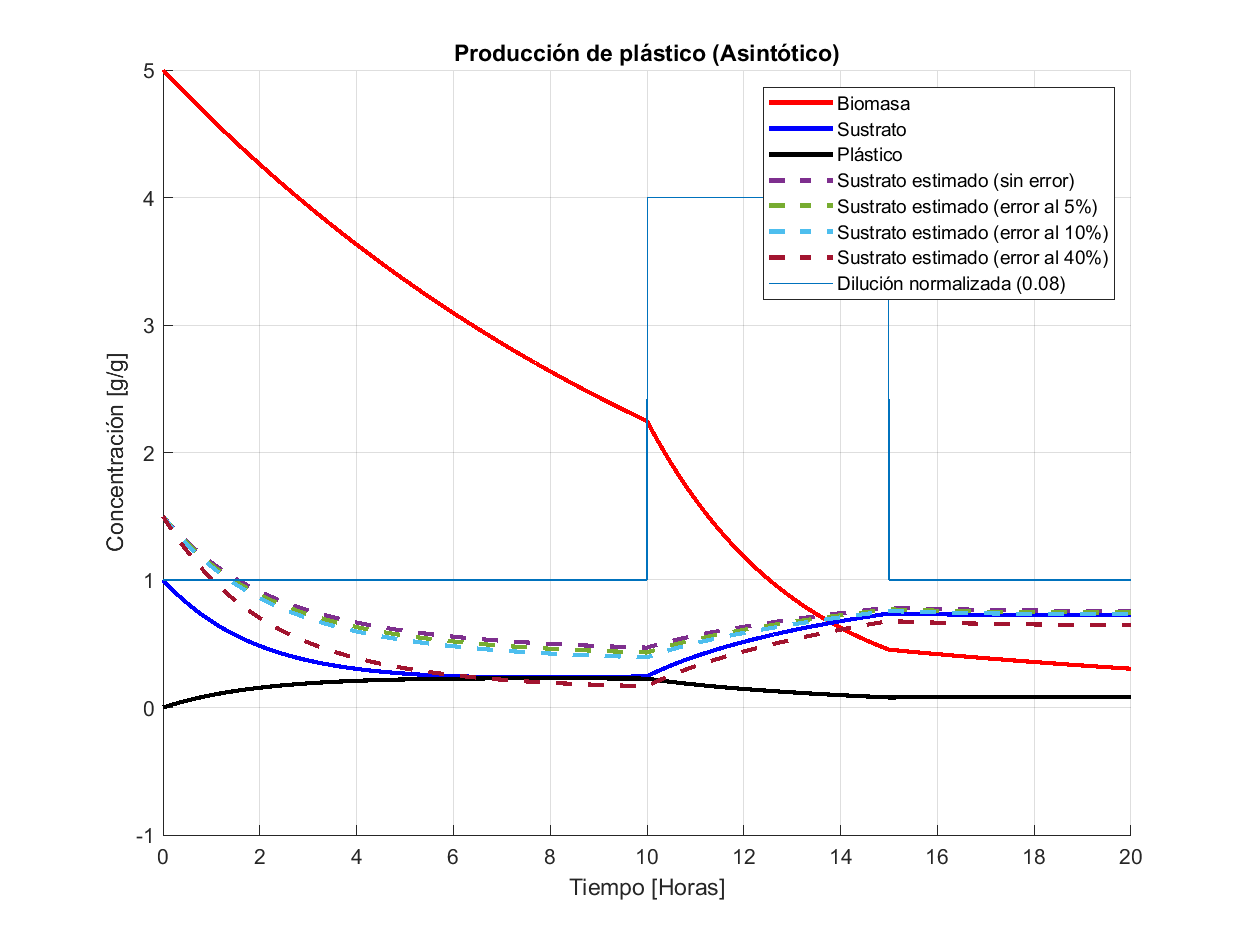
\includegraphics[width=0.43\textwidth]{./Images_tp2/asintotico.png}
  \caption{Observador asintótico con variaciones en $K_{s2}$}
\end{figure}

\begin{figure}[H]
  \centering
  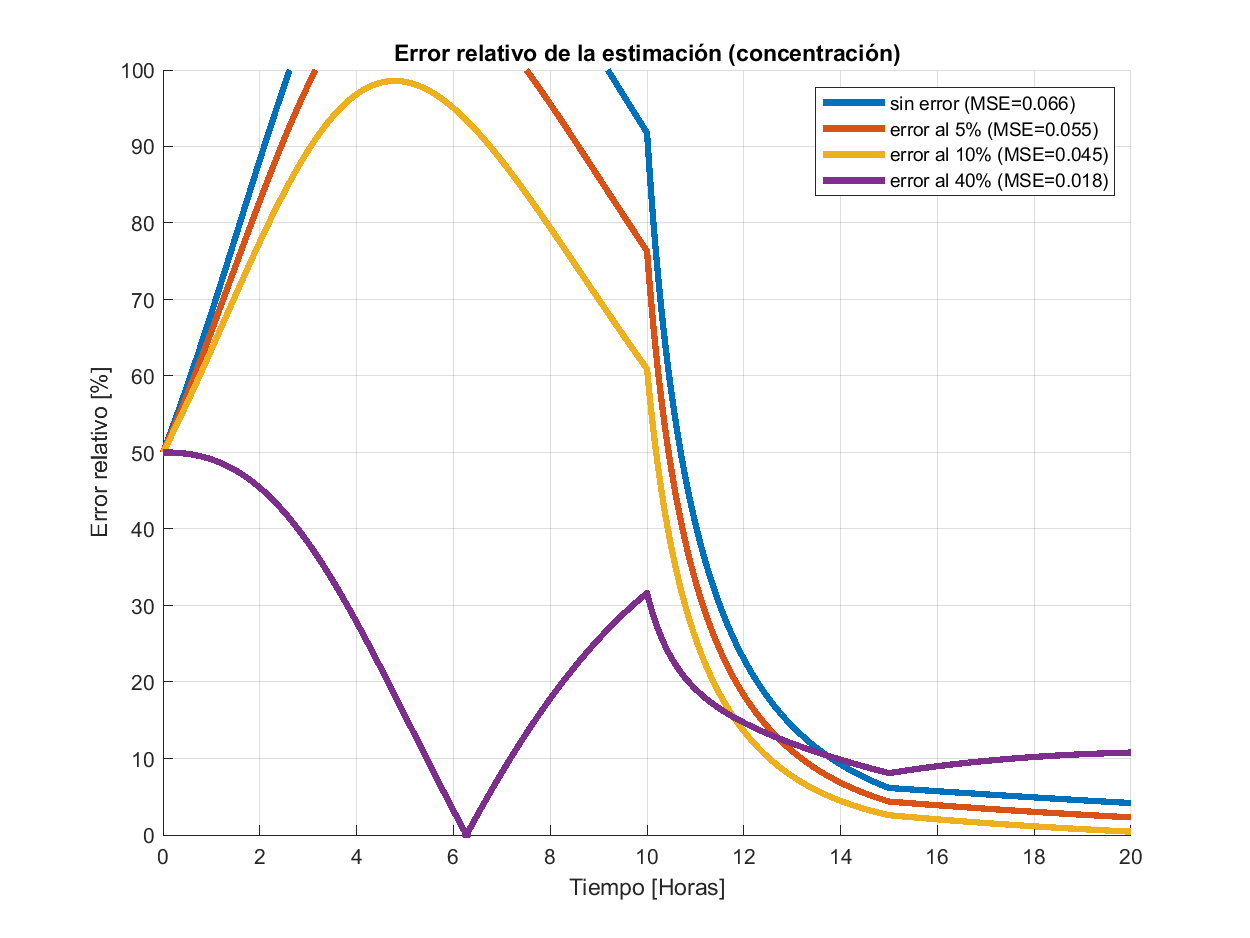
\includegraphics[width=0.43\textwidth]{./Images_tp2/asintotico_error.png}
  \caption{Error relativo del observador asintótico}
\end{figure}

\section{Conclusiones}

Tras comparar los tres observadores, se concluye que:

\begin{itemize}
  \item{Observador exponencial: Requiere sintonización manual de polos y es vulnerable a incertidumbres paramétricas, aunque converge en estado estacionario.}
  \item{EKF: Ofrece estimaciones óptimas en entornos ruidosos, pero su complejidad computacional limita su escalabilidad.}
  \item{Observador asintótico: Destaca como la mejor opción para este sistema. Su independencia del modelo (excepto $K_{s2}$), convergencia a error cero y robustez frente a perturbaciones lo hacen ideal para implementación práctica.}
\end{itemize}


\end{document}